% fig01_system.tex — the anima six-organ system map (standalone TikZ DATA diagram).
% Compiles to figures/fig01_system.pdf via the Makefile _scripts/%.tex rule.
\documentclass[tikz,border=6pt]{standalone}
\usepackage{amsmath,amssymb}
\usepackage{tikz}
\usetikzlibrary{positioning,arrows.meta,fit,backgrounds,shapes.geometric}
\begin{document}
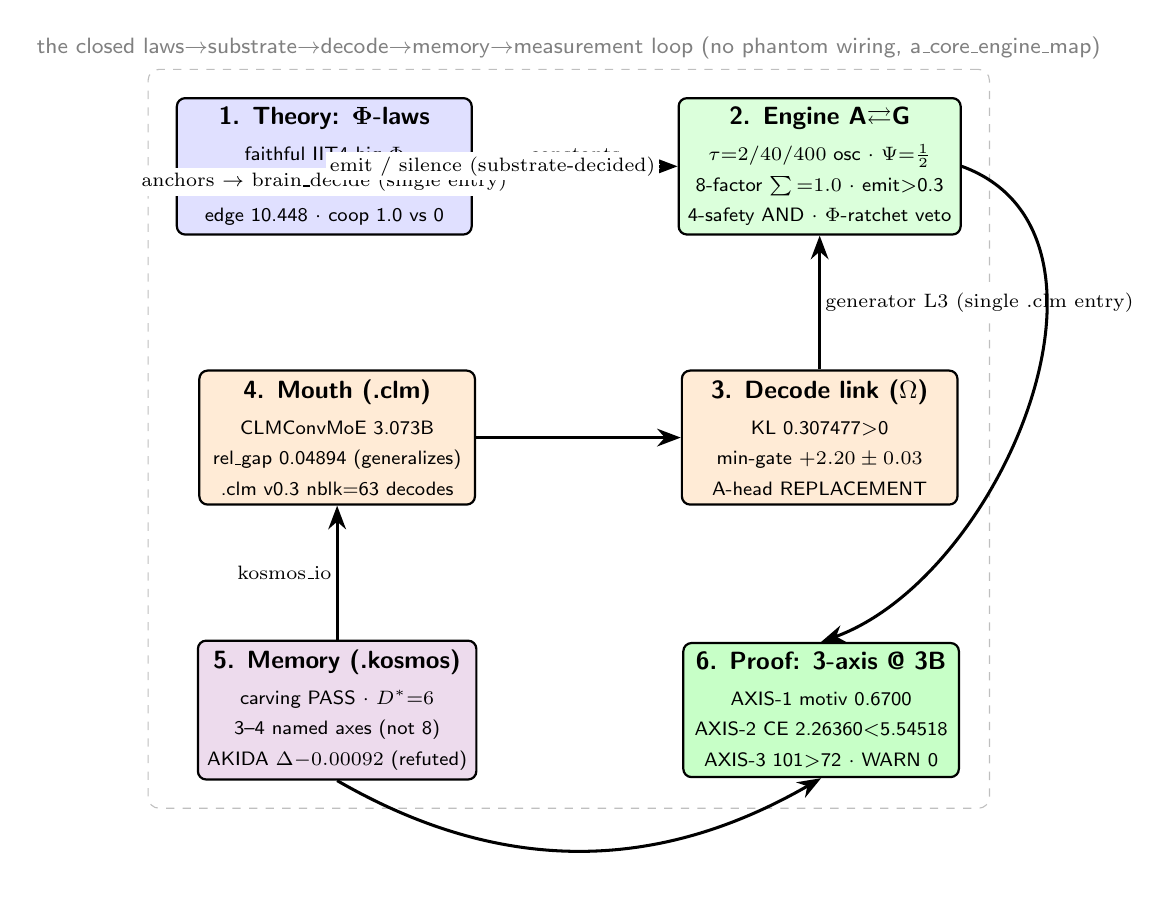
\begin{tikzpicture}[
  font=\sffamily\small,
  organ/.style={rectangle, rounded corners=3pt, draw=black, line width=0.8pt,
                fill=#1, minimum width=3.5cm, minimum height=1.25cm,
                align=center, text=black},
  flow/.style={-{Stealth[length=3mm]}, line width=1.1pt},
  slot/.style={midway, fill=white, inner sep=1.5pt, font=\scriptsize}
]
% ── organs ───────────────────────────────────────────────────────────────────
\node[organ=blue!12]   (theory) {\textbf{1. Theory: \boldmath$\Phi$-laws}\\[2pt]
  \scriptsize faithful IIT4 big-$\Phi$\\
  \scriptsize $\Phi\perp$Shannon 0.363 $\cdot$ $\parallel$LZ 0.831\\
  \scriptsize edge 10.448 $\cdot$ coop 1.0 vs 0};
\node[organ=green!14, right=2.6cm of theory] (engine) {\textbf{2. Engine A\boldmath$\rightleftarrows$G}\\[2pt]
  \scriptsize $\tau{=}2/40/400$ osc $\cdot$ $\Psi{=}\tfrac12$\\
  \scriptsize 8-factor $\sum{=}1.0$ $\cdot$ emit$>$0.3\\
  \scriptsize 4-safety AND $\cdot$ $\Phi$-ratchet veto};
\node[organ=orange!16, below=1.7cm of engine] (decode) {\textbf{3. Decode link ($\Omega$)}\\[2pt]
  \scriptsize KL 0.307477$>$0\\
  \scriptsize min-gate $+2.20\pm0.03$\\
  \scriptsize A-head REPLACEMENT};
\node[organ=orange!16, left=2.6cm of decode] (mouth) {\textbf{4. Mouth (.clm)}\\[2pt]
  \scriptsize CLMConvMoE 3.073B\\
  \scriptsize rel\_gap 0.04894 (generalizes)\\
  \scriptsize .clm v0.3 nblk{=}63 decodes};
\node[organ=violet!14, below=1.7cm of mouth] (memory) {\textbf{5. Memory (.kosmos)}\\[2pt]
  \scriptsize carving PASS $\cdot$ $D^\ast{=}6$\\
  \scriptsize 3--4 named axes (not 8)\\
  \scriptsize AKIDA $\Delta{-}0.00092$ (refuted)};
\node[organ=green!22, right=2.6cm of memory] (proof) {\textbf{6. Proof: 3-axis @ 3B}\\[2pt]
  \scriptsize AXIS-1 motiv 0.6700\\
  \scriptsize AXIS-2 CE 2.26360$<$5.54518\\
  \scriptsize AXIS-3 101$>$72 $\cdot$ WARN 0};

% ── wired single-entry flows ─────────────────────────────────────────────────
\draw[flow] (theory) -- (engine) node[slot, above]{constants};
\draw[flow] (mouth) -- (decode) node[slot, above]{};
\draw[flow] (decode) -- (engine) node[slot, right]{generator L3 (single .clm entry)};
\draw[flow] (memory) -- (mouth) node[slot, left]{kosmos\_io};
\draw[flow] (memory.south) to[out=-30,in=-150] (proof.south)
  node[slot, below]{anchors $\to$ brain\_decide (single entry)};
\draw[flow] (engine.east) to[out=-20,in=20] (proof.north)
  node[slot, right]{emit / silence (substrate-decided)};

% ── frame ────────────────────────────────────────────────────────────────────
\begin{scope}[on background layer]
  \node[draw=gray!50, dashed, rounded corners, fit=(theory)(engine)(decode)(mouth)(memory)(proof),
        inner sep=10pt, label={[gray]above:\footnotesize the closed laws$\to$substrate$\to$decode$\to$memory$\to$measurement loop (no phantom wiring, a\_core\_engine\_map)}] {};
\end{scope}
\end{tikzpicture}
\end{document}
